% !TEX encoding = UTF-8
% !TEX TS-program = pdflatex
% !TEX root = ../tesi.tex

%**************************************************************
\chapter{L'applicazione}
\label{cap:applicazione}
%**************************************************************

%\intro{Breve introduzione al capitolo}\\

\section{Introduzione alle grammatiche}
Zucchetti negli ultimi anni ha investito molto nella ricerca di una tecnologia che gli permettesse di interagire con i propri prodotti attraverso comandi vocali ed ora sta realizzando delle regole per generare \emph{grammatiche} capaci di comprendere ed elaborare un numero potenzialmente infinito di frasi del linguaggio naturale. \\
Gli assistenti virtuali presenti sul mercato sono basati sul seguente concetto: provare in ogni modo ad interpretare l'input ricevuto anche se non corrisponde esattamente ad uno di quelli previsti, a costo di commettere degli errori. L'obiettivo di questa filosofia è dare all'utente la percezione di utilizzare uno strumento in grado di capire e ragionare in qualsiasi condizione ed è già utilizzata in larga scala da aziende del calibro di Google, Amazon e Apple. Tuttavia, per le funzionalità offerte dalla maggior parte dei prodotti Zucchetti, tale principio non è applicabile poiché necessitano che la comprensione dell'input abbia margine di errore nullo. Un classico esempio è il trasferimento di denaro in cui se la comprensione del comando avviene in modo errato c'è il rischio di causare danni contingenti agli utenti. \\
Zucchetti ha perciò intrapreso una strada diversa sviluppando una tecnologia che si pone l'obiettivo di massimizzare la precisione nella comprensione dei comandi, accettando piuttosto di rigettarli qualora non abbia la piena certezza. Essa consiste in regole molto semplici ed intuitive da applicare e riassunte in cinque operazioni chiave:
\begin{itemize}
	\item concatenazione di stringhe;
	\item scelta tra più stringhe;
	\item ripetizione di uno o più stringhe;
	\item opzionalità di una stringa;
	\item rilascio di una stringa a scelta dello sviluppatore in qualsiasi punto dell'interpretazione come segnale per l'elaborazione dei risultati.
\end{itemize}
A partire da esse viene costruita una \emph{\gls{gramg}} che permette di interpretare un insieme finito di input rappresentanti il dominio della conversazione che si vuole intrattenere. La difficoltà principale è scegliere il corretto insieme delle possibili frasi che l'utente può pronunciare con l'obiettivo di ottenerne un numero elevato ma pertinente, eseguendo un'analisi probabilistica e statistica sul proprio contesto. Il problema infatti è che, qualora l'utente esprimesse una frase che differisca anche per una singola lettera da quelle generate dalla \emph{\gls{gramg}}, non sarebbe riconosciuta. \\
Un esempio semplice ma dimostrativo di una \emph{\gls{gramg}} che permette di interpretare alcune frasi di saluto è illustrato nella seguente immagine.

\begin{figure}[htbp]
	\begin{center}
		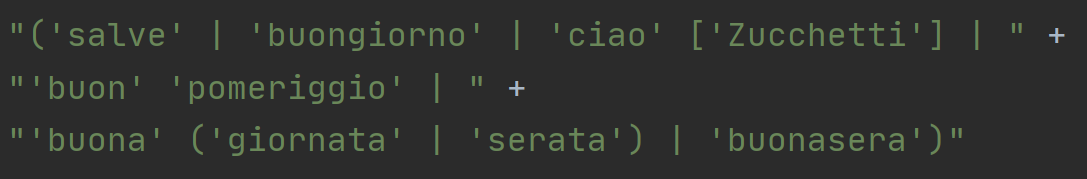
\includegraphics[height=1.8cm, width=\linewidth]{esempio-grammatica.PNG}
		\caption{Esempio di una grammatica}
	\end{center}
\end{figure}

\vspace{2cm}

Nonostante il loro principio di funzionamento sia relativamente semplice da comprendere, non sono altrettanto facili da interpretare se raggiungono grandi dimensioni, soprattutto per uno sviluppatore terzo che le dovrà riutilizzare in futuro. Per migliorare questo aspetto l'azienda ha deciso di utilizzare i diagrammi \emph{\gls{rldg}}\glsfirstoccur come strumento di rappresentazione come si può vedere nella figura successiva.

\begin{figure}[htbp]
	\begin{center}
		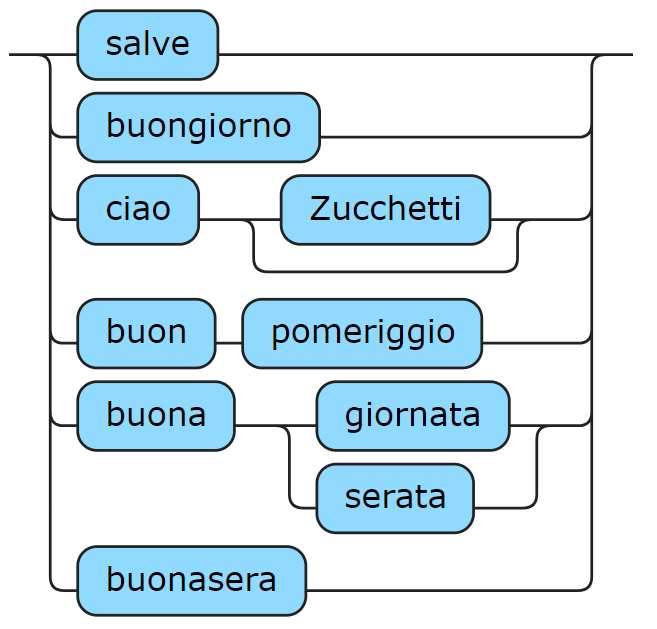
\includegraphics[height=6cm]{esempio-railroad.PNG}
		\caption{Esempio di una grammatica con railroad}
	\end{center}
\end{figure}

Risulta evidente infatti come questa raffigurazione sia molto più efficace e intuitiva. \\
Inoltre l'applicazione effettiva della \emph{\gls{gramg}} sugli input dell'utente avviene attraverso un apposito \emph{\gls{parsg}}\glsfirstoccur che mi è stato consegnato dall'azienda per lo sviluppo del progetto. \\
Infine per riassumere gli aspetti positivi e negativi di questa tecnologia viene presentato un paragone a quella attualmente utilizzata dagli assistenti virtuali presentati in precedenza. Non tutti i paragoni sono possibili a causa della mancanza di dati a disposizione ma viene comunque riportato nella seguente tabella.

%\begin{table}
	\begin{longtable}{|p{3cm}|p{4.5cm}|p{4.5cm}|}
		\hline
		\textbf{Caratteristica} & \textbf{Zucchetti} & \textbf{Aziende concorrenti} \\\hline
		
		Precisione nella comprensione & Estrema precisione: quando è compresa una frase si ha la certezza di averlo fatto correttamente.  & Buona precisione: quando è compresa una frase si ha buone probabilità di averlo fatto correttamente ma non la certezza. \\
		\hline
		Propensione alla comprensione & Comprende solo le frasi che lo sviluppatore mette a disposizione attraverso una \emph{\gls{gramg}}. & Cerca di interpretare anche frasi che non corrispondono esattamente a quelle a disposizione, talvolta commettendo degli errori. \\
		\hline
		Verbosità nello sviluppo & Poca verbosità in quanto, per costruzione, ad un aumento minimale vocaboli si ottiene un grande aumento delle frasi potenzialmente interpretabili. & Dati non disponibili. \\
		\hline
		Facilità della sintassi & Molto facili da gestire in quanto è basata su regole semplici che permettono di produrre molte frasi. & Dati non disponibili. \\
		\hline
		Prestazioni & Prestazioni molto elevate dovute ad un'ottima integrazione del \emph{\gls{parsg}} e all'esecuzione in locale, senza quindi onere nella comunicazione. & Prestazioni altrettanto elevate con l'incognita dei tempi di latenza dovuti all'esecuzione in remoto del \emph{\gls{parsg}} di interpretazione dell'input. \\
		\hline
		\caption{Tabella di confronto tra la tecnologia Zucchetti e quella dei concorrenti per l'interpretazione del linguaggio naturale}
	\end{longtable}
%\end{table}

\section{Analisi dei requisiti}
	\subsection{Descrizione del problema}
	Durante l'attività di ricerca sugli assistenti virtuali, in particolare nello sviluppo del \emph{\gls{pocg}} che fa uso di Alexa, è emerso un concetto importante, caratteristico anche del lavoro che sta svolgendo l'azienda: la conversazionalità. Essa rappresenta la capacità di intrattenere una conversazione da parte di un software simulando la presenza di una persona. \\
	Inoltre nella pianificazione del lavoro è inserita la costruzione di una \emph{\gls{nlug}} con relativa \emph{\gls{gramg}} che interpreti un insieme di frasi e dia una risposta ragionata sulla base di esse. \\
	È stato quindi deciso, in comune accordo con il tutor, di costruire un'applicazione che metta assieme la realizzazione di una propria \emph{\gls{nlug}} con capacità di conversazione finalizzata a soddisfare una determinata funzionalità e non limitata ad una coppia domanda-risposta. Il dominio dell'applicazione è simile a quello del \emph{\gls{pocg}} sviluppato con Alexa ovvero la data di nascita, solo che molto più completo. Le frasi pronunciabili dagli utenti per cui è prevista la comprensione sono  composte da:
	\begin{itemize}
		\item saluto iniziale opzionale;
		\item un insieme di frasi introduttive per esprimere la data di nascita nel formato giorno, mese e anno o, alternativamente, la data di compleanno nel formato giorno, mese;
		\item insieme di espressioni per la data di nascita e conseguentemente del sottoinsieme data di compleanno;
		\item insieme di frasi per riconoscere come data le espressioni che definiscono il giorno di Natale;
		\item insieme di frasi per riconoscere come data le espressioni che definiscono il primo giorno di un qualsiasi mese;
		\item insieme di frasi per interrompere l'esecuzione in qualunque momento;
		\item insieme di frasi per chiedere un eventuale aiuto sulle funzionalità offerte dell'applicazione.
	\end{itemize}
	\subsection{Requisiti}
	Lo scopo principale è dimostrare la fattibilità di implementare la capacità conversazionale in una \emph{\gls{nlug}} costruita con la tecnologia sviluppata da Zucchetti. L'applicazione perciò si presenta sotto forma di \emph{\gls{pocg}} e non è quindi integrata in un software aziendale esistente. \\
	Analizzando più in dettaglio gli obiettivi da raggiungere, è stata stilata una lista di requisiti obbligatori la cui fattibilità è certa. Uno tra quelli emersi, invece, è stato inserito come opzionale poiché rappresenta un miglioramento ragionevolmente non implementabile nel tempo a disposizione.
	I requisiti obbligatori sono i seguenti:
	\begin{enumerate}
		\item costruzione di una \emph{\gls{nlug}} che comprenda la data di nascita espressa dall'utente, esegua un'elaborazione e prepari una risposta adatta. Deve avere estrema precisione nella comprensione delle le frasi anche a costo di rigettarne alcune;
		\item implementazione della capacità conversazionale con relativa memoria che permetta di portare a compimento l'attività in esecuzione, provando a dare la percezione all'utente di dialogare con una persona. Più in dettaglio consiste nel richiedere i componenti mancanti della data di nascita o di compleanno oppure nella modifica dovuto a possibili errori, affinché l'utente li fornisca in modo completo e corretto;
		\item costruzione dell'interfaccia utente composta da:
		\begin{itemize}
			\item interfaccia grafica minimale che permetta all'utente di attivare il riconoscimento della voce;
			\item interfaccia vocale completa di tutti gli accessori studiati durante l'attività di ricerca. In input risulta essere una diretta conseguenza dello sviluppo della \emph{\gls{nlug}} mentre in output è progettata sulla base delle elaborazioni prodotte.
		\end{itemize}
	\end{enumerate}
	Il requisito opzionale è il seguente:
	\begin{enumerate}
		\item generalizzazione della grammatica che permetta non solo di interpretare l'input dell'utente ma anche di generare le risposta adeguate sulla base dell'elaborazione.
	\end{enumerate}
\section{Progettazione}
	\subsection{NLU}
	La \emph{\gls{nlug}} è il nucleo di tutto l'applicativo e la sua corretta progettazione è fondamentale. Essa consiste nella generazione di una \emph{\gls{gramg}} che interpreta l'input dell'utente e nella sua applicazione alle stringhe di testo. La \emph{\gls{gramg}} non è rappresentabile in un unico diagramma \emph{\gls{rldg}} in quanto ha dimensioni troppo elevate perciò sono illustrate le parti fondamentali. \\
	Il seguente diagramma rappresenta l'insieme di frasi per richiedere la data di nascita in cui prima viene detto il frammento di frase che corrisponde all'introduzione del contenuto come ad esempio "sono nato il" oppure "la mia data di nascita è" e successivamente il contenuto vero e proprio ovvero giorno, mese e anno in tutte le possibili combinazioni. 
		
	\begin{figure}[htbp]
		\begin{center}
			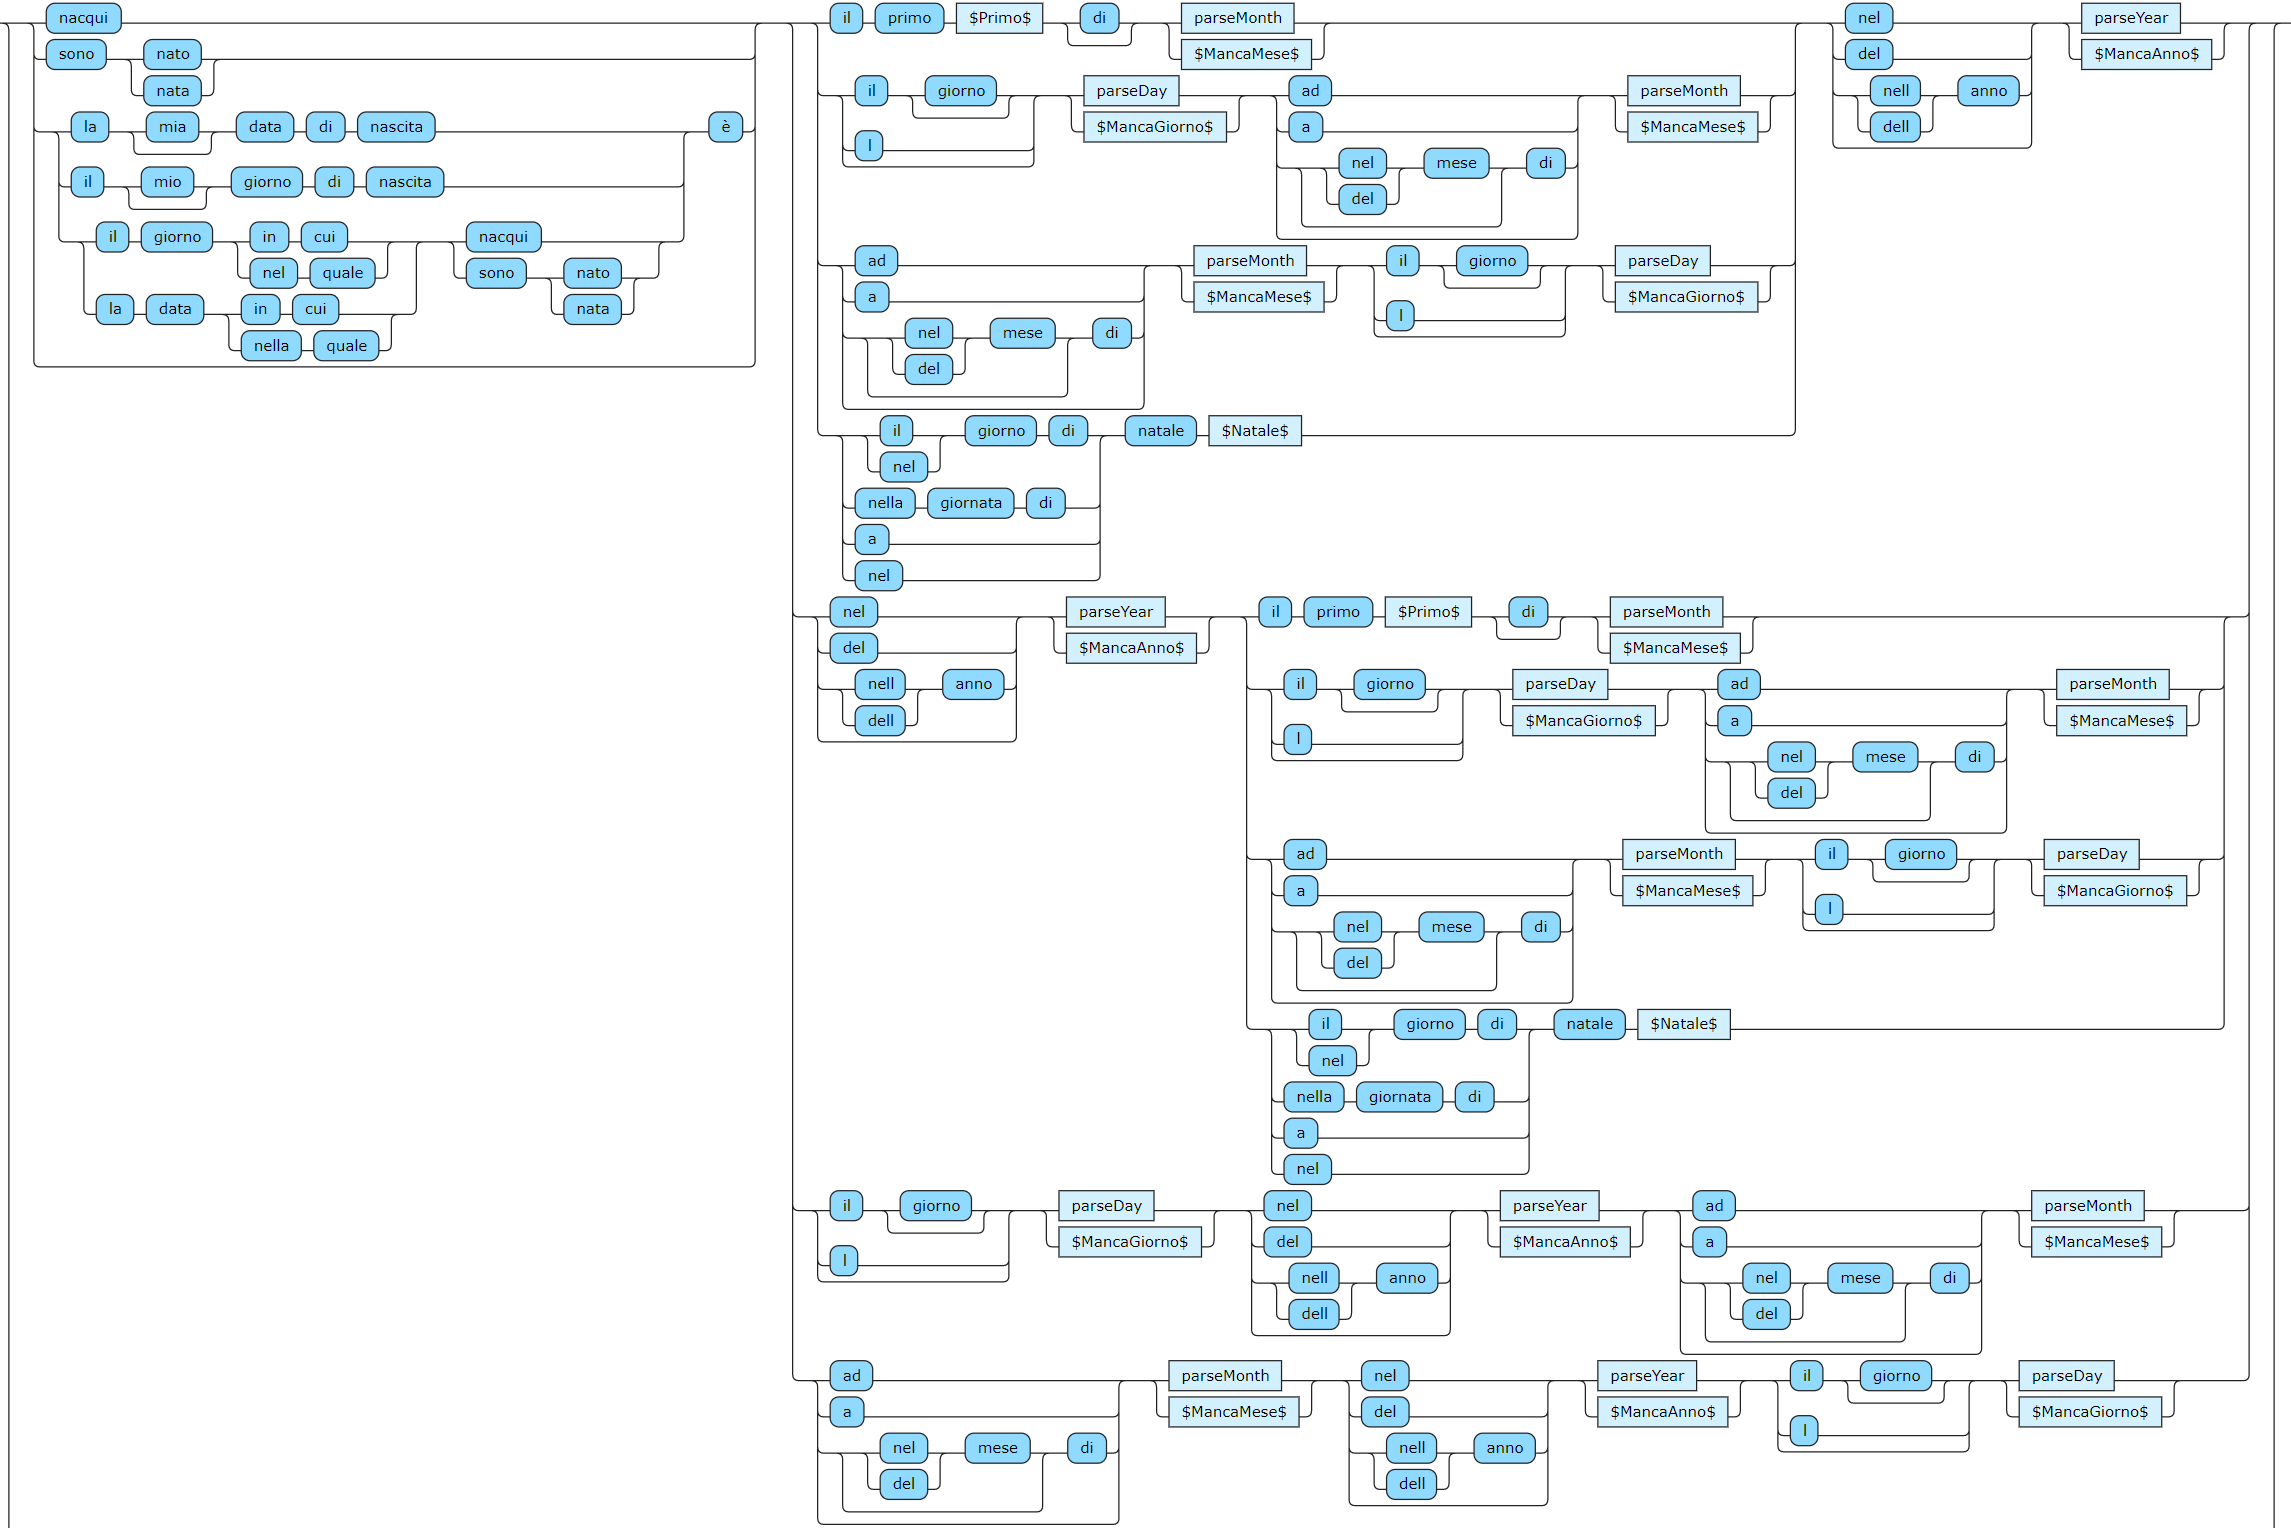
\includegraphics[height=12cm, width=\linewidth]{railroad_data_nascita.png}
			\caption{Diagramma railroad della grammatica per la data di nascita prima parte}
		\end{center}
	\end{figure}

	\pagebreak
	
	Nella figura successiva invece è rappresentato il diagramma \emph{\gls{rldg}} opposto in cui prima è previsto il contenuto ovvero giorno, mese e anno, sempre in tutte le possibili combinazioni, ed in seguito le sue frasi introduttive. Questo permette di riconoscere un maggior numero di versioni in cui l'utente può esprimere la data di nascita.
	
	\begin{figure}[htbp]
		\begin{center}
			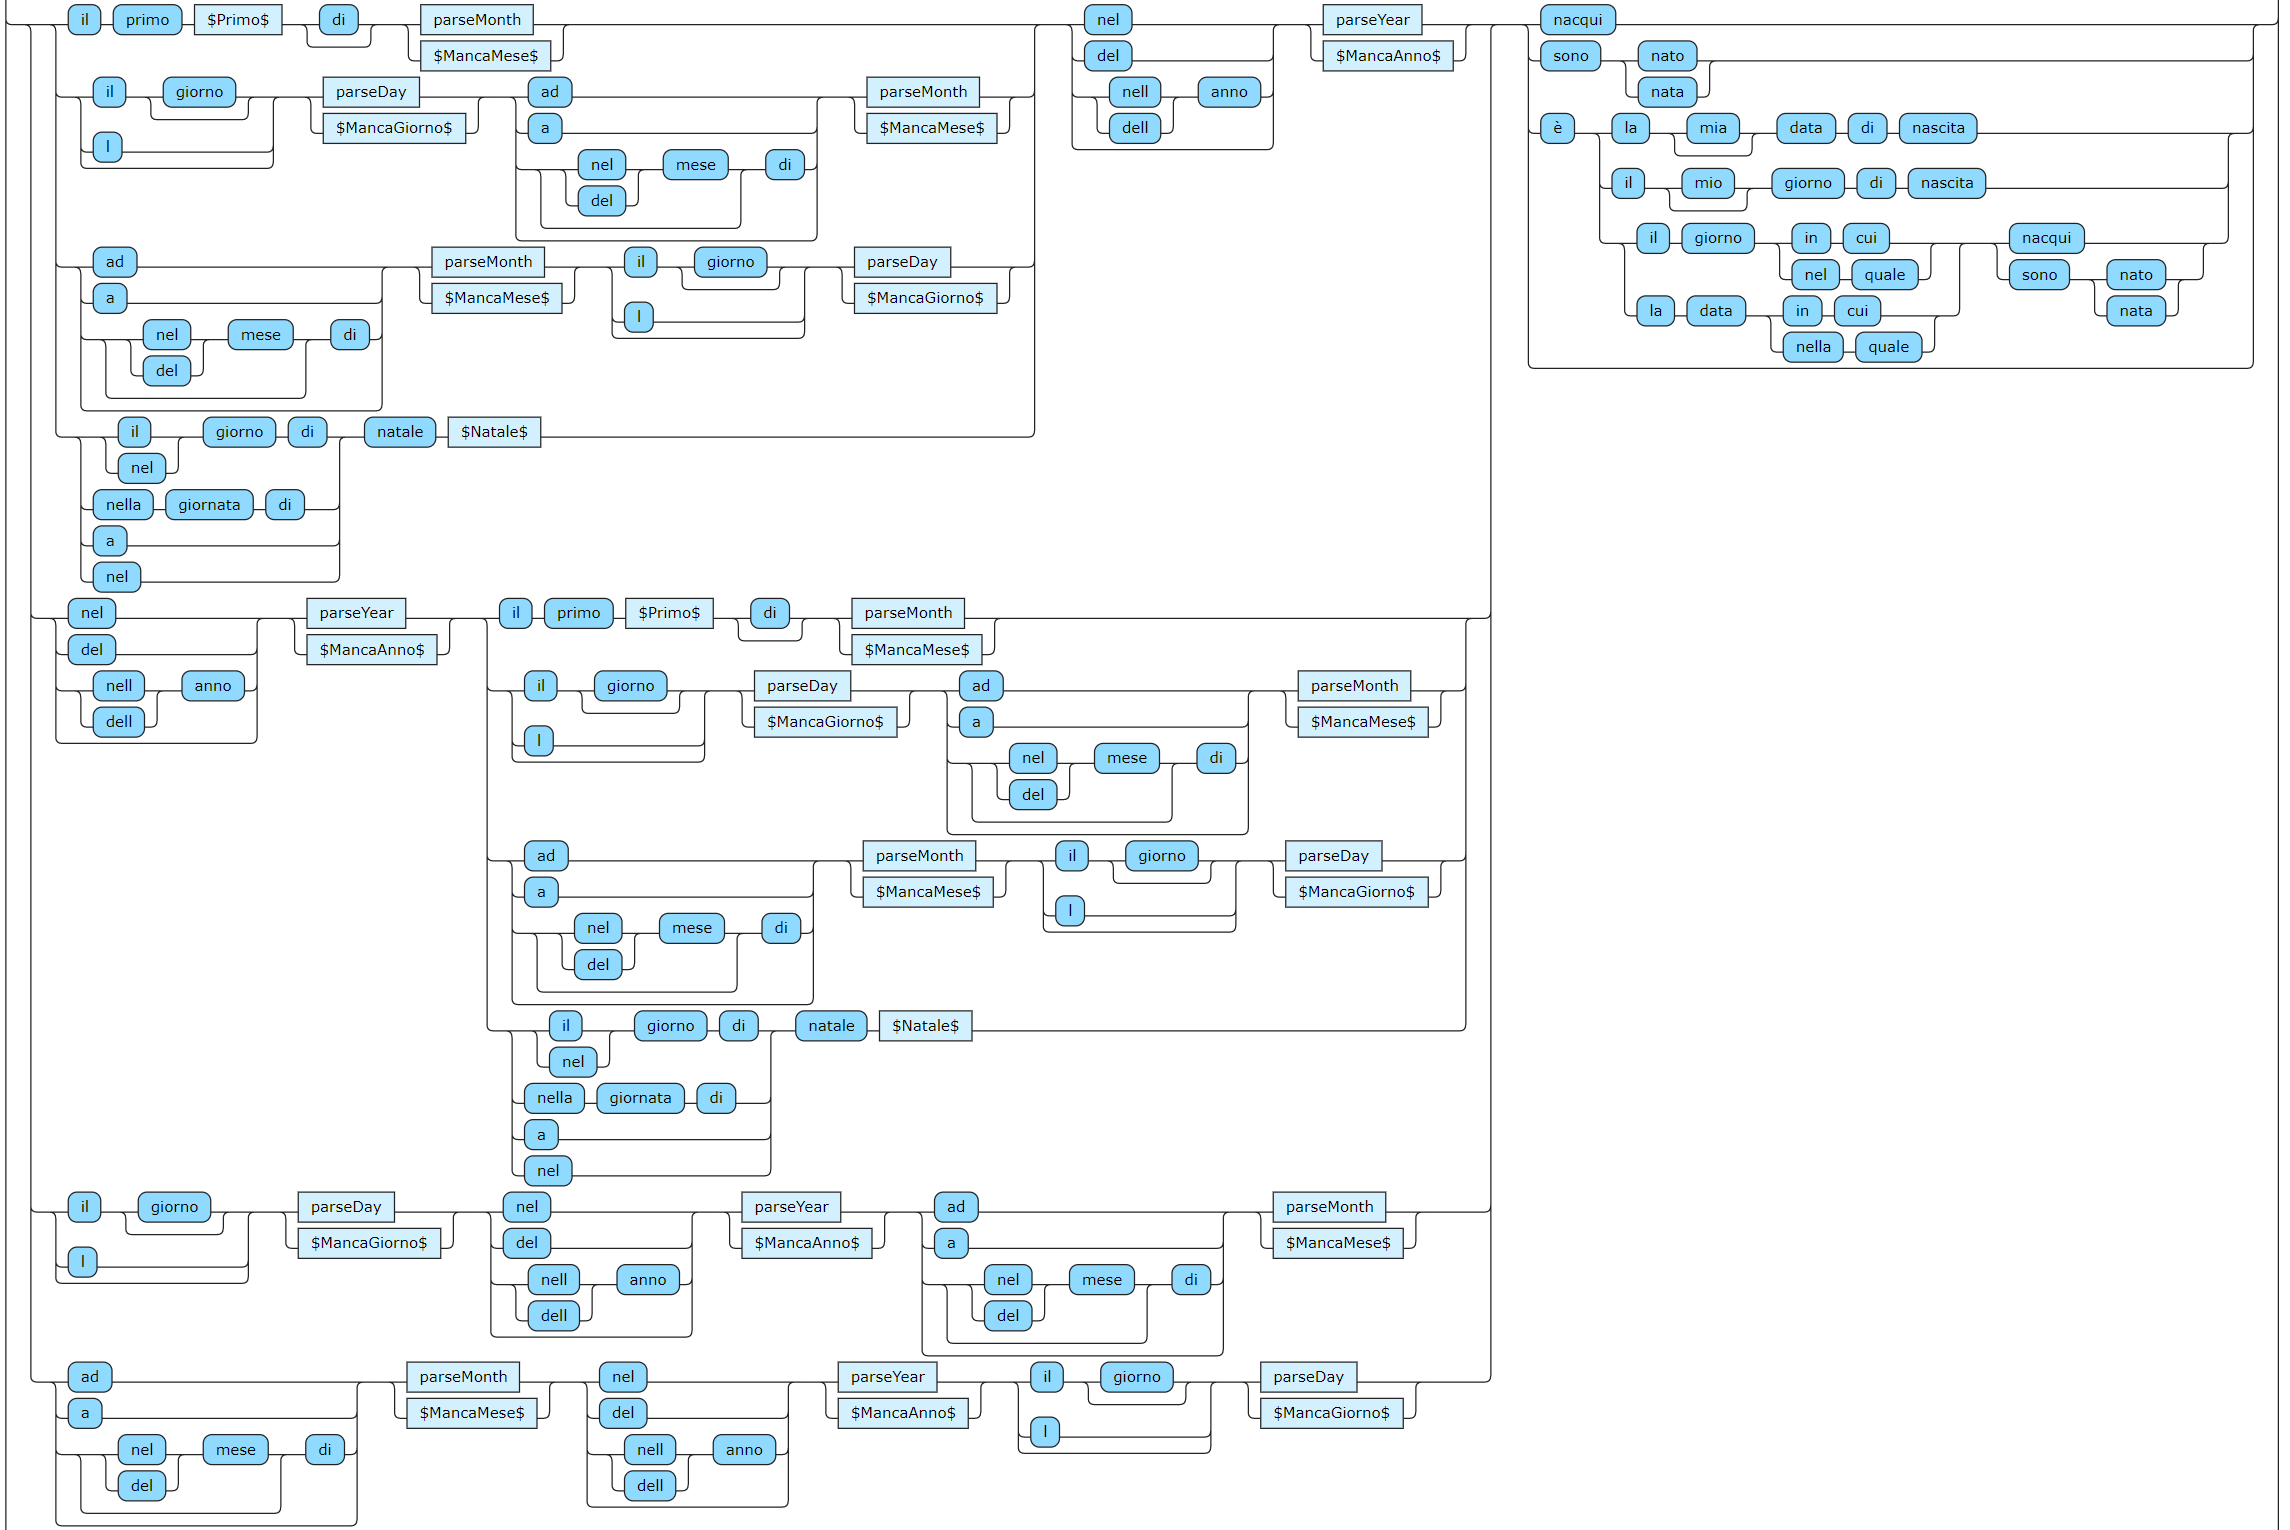
\includegraphics[height=12cm, width=\linewidth]{railroad_data_nascita_2.png}
			\caption{Diagramma railroad della grammatica per la data di nascita seconda parte}
		\end{center}
	\end{figure}

	Le due porzioni di \emph{\gls{gramg}} illustrate permettono globalmente di interpretare la data di nascita. Successivamente, seguendo lo stesso principio di separazione tra i frammenti di frase introduttivi e quelli di contesto, sono presentate le due porzioni di \emph{\gls{gramg}} che illustrano la data di compleanno, differente dalla precedente per l'assenza dell'anno. \\
	La figura seguente riporta la porzione che presenta prima la parte introduttiva e dopo quella di contenuto.
	
	\begin{figure}[htbp]
		\begin{center}
			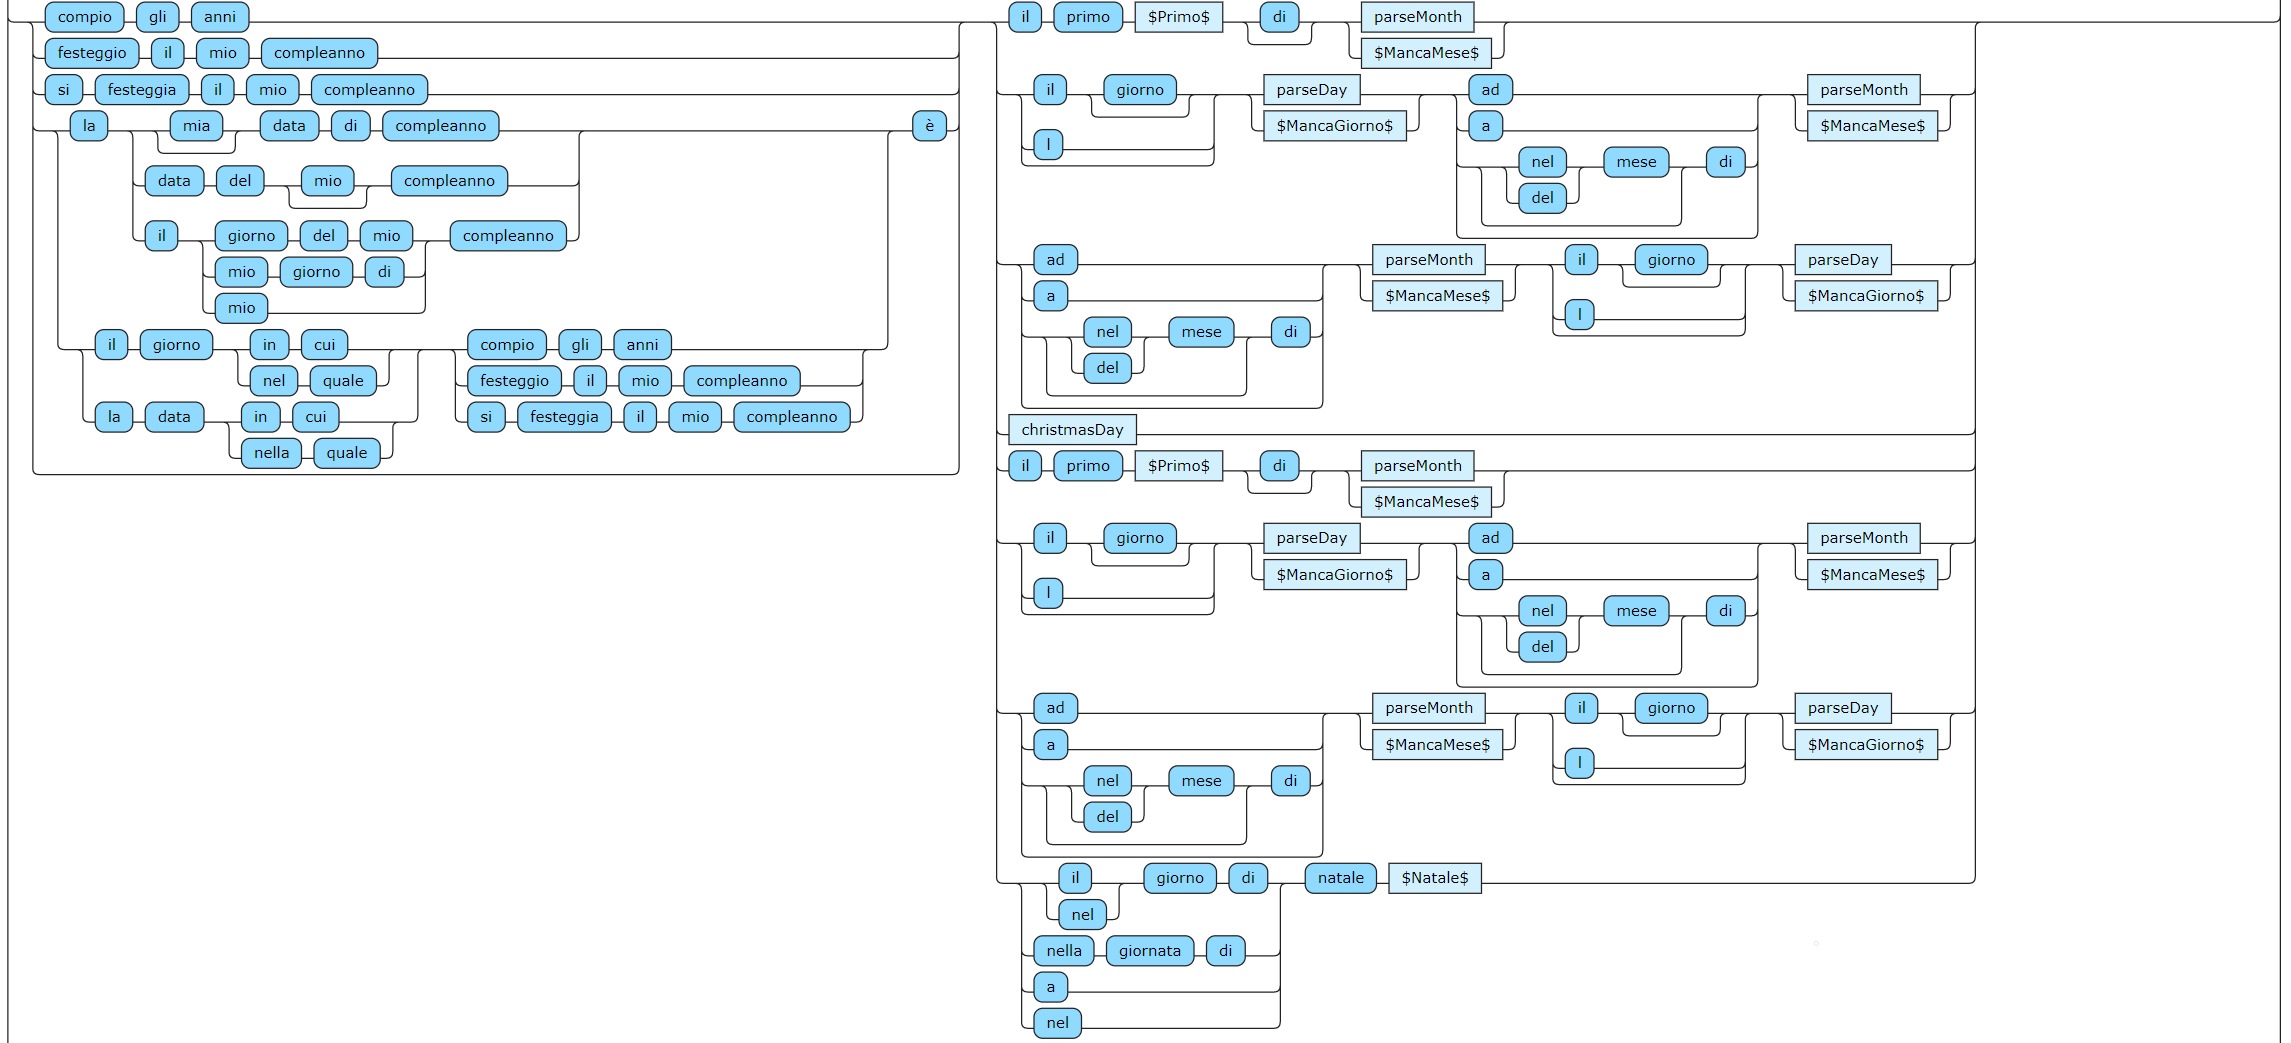
\includegraphics[height=9cm, width=\linewidth]{railroad_compleanno.png}
			\caption{Diagramma railroad della grammatica per il compleanno prima parte}
		\end{center}
	\end{figure}
	\pagebreak

	La prossima figura, invece, riporta la porzione che presenta prima la parte di contenuto e dopo quella introduttiva.
	\begin{figure}[htbp]
		\begin{center}
			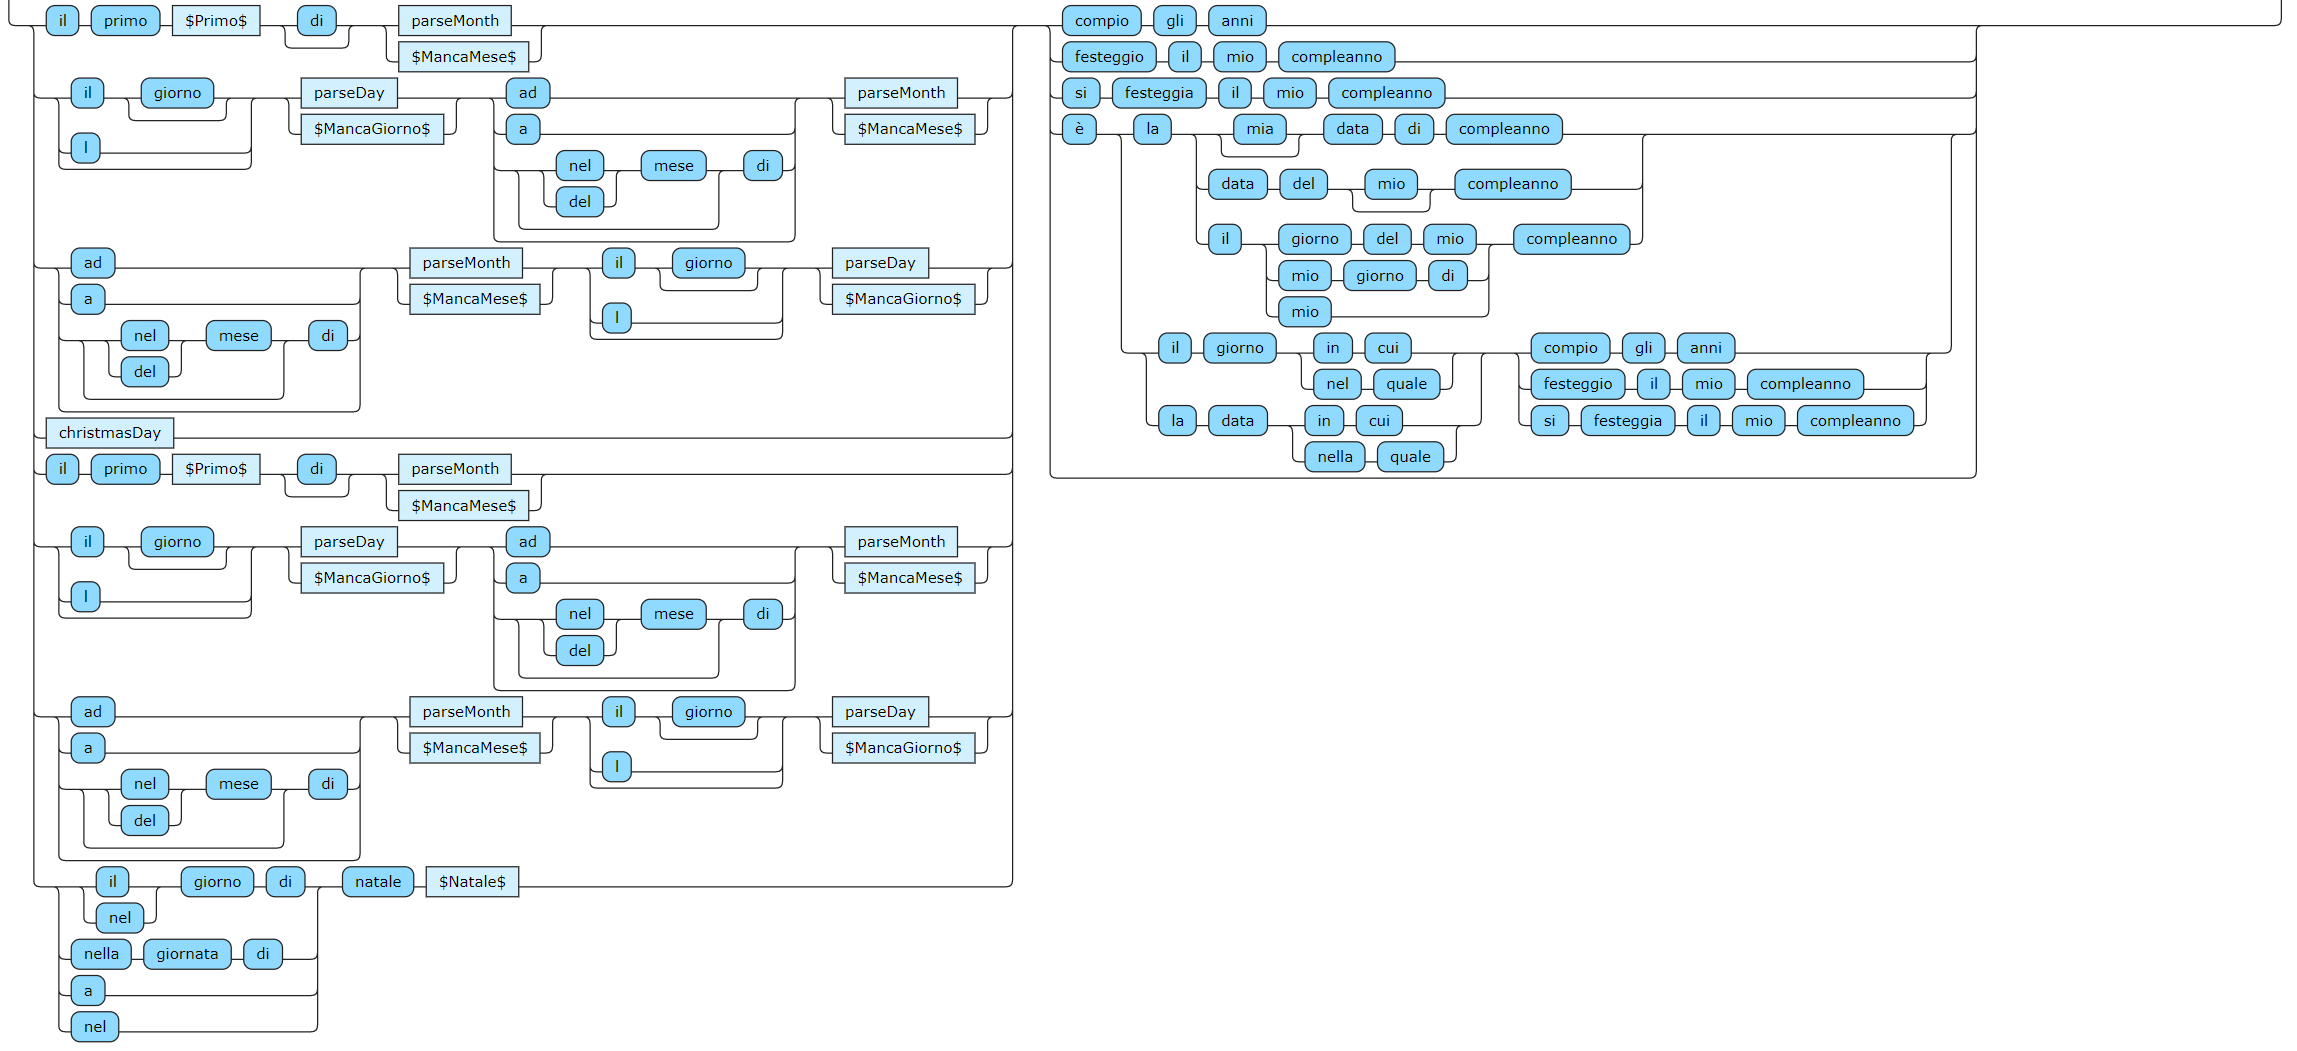
\includegraphics[height=9cm, width=\linewidth]{railroad_compleanno_2.png}
			\caption{Diagramma railroad della grammatica per il compleanno seconda parte}
		\end{center}
	\end{figure}
	\pagebreak

	\subsection{Capacità conversazionale}
	Nella progettazione della capacità conversazionale il concetto fondamentale è la memoria. Infatti, mentre la \emph{\gls{nlug}} permette l'interpretazione del linguaggio naturale, la capacità conversazionale consente di mantenere il contesto durante l'intero dialogo. \\
	Ho deciso di tenere traccia dei dati che lo costituiscono all'interno di un oggetto che sarà resettato ad ogni nuova conversazione. In questo modo è possibile costruire delle risposte basate sul contesto per porre domande mirate ad ottenere eventuali dati mancanti ovvero giorno, mese e anno. \\
	Infine per l'implementazione della conversazione è sufficiente implementare la \emph{\gls{gramg}} descritta in precedenza in quanto è stata progettata anche per riconoscere singole parti di contenuto. \\
	Per un ulteriore migliramento sarebbe stato possibile tenere traccia dei dati forniti dall'utente in modo permanente, ad esempio in un database, così che ad un nuovo utilizzo dell'utente, anche a distanza di tempo, l'applicazione si ricordasse di ciò che era stato detto in precedenza e potesse riprende la conversazione. Questo però avrebbe comportato alcuni vincoli quali, ad esempio, la realizzazione di un sistema di autenticazione, diventando troppo complesso nel tempo a disposizione. 
	\subsection{Interfaccia utente}
	La progettazione dell'interfaccia utente si articola in due parti:
	\begin{itemize}
		\item interfaccia grafica;
		\item interfaccia vocale.
	\end{itemize}
		\subsubsection{Interfaccia grafica}
		L'interfaccia grafica è stata progettata con un numero di elementi minimali all'interno ed è illustrata nella seguente immagine.
		\begin{figure}[htbp]
			\begin{center}
				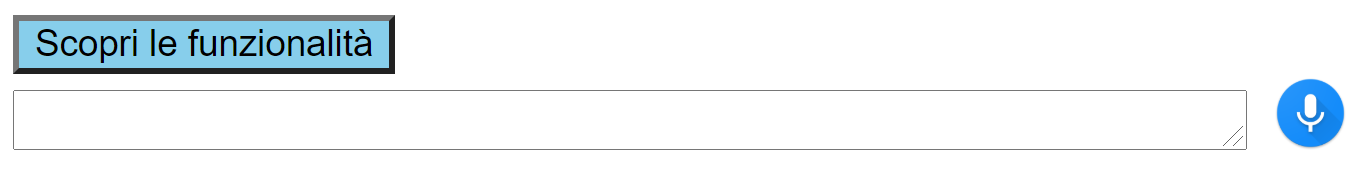
\includegraphics[height=1.7cm, width=\linewidth]{interfaccia-grafica.PNG}
				\caption{Interfaccia grafica dell'applicazione}
			\end{center}
		\end{figure}
	
		I componenti sono un pulsante che permette all'utente di ascoltare le funzionalità fornite, un pulsante con l'immagine del microfono che attiva il riconoscimento vocale ed una casella di testo non editabile che permetta di visualizzare il comando che è stato riconosciuto.		
		\subsubsection{Interfaccia vocale}
		L'interfaccia vocale è stata progettata con l'obiettivo di garantire la migliore esperienza possibile d'uso agli utenti. \\
		Ho utilizzato le nozioni apprese dalla documentazione degli assistenti virtuali analizzati per generare un'interfaccia vocale e sono:
		\begin{itemize}
			\item capire la tipologia degli utenti che deve interagire con la propria applicazione. In questo caso ha avuto importanza relativa in quanto si tratta di un \emph{\gls{pocg}} e non è stata prevista una categoria specifica;
			\item provare a costruire esempi di dialogo molteplici verificando quali risultano più naturali su un insieme di persone sia del team di sviluppo sia di altri impieghi. Nel mio caso l'ho provato con alcuni colleghi e persone esterne;
			\item scegliere uno stile di conversazione che si adatti maggiormente al contesto della propria applicazione;
			\item dare una spiegazione iniziale di ciò che si può dire o fare in caso di interfaccia grafica ausiliaria;
			\item valutare l'utilizzo di un'interfaccia grafica di ausilio per mantenere meglio il contesto, soprattutto se risulta corposo;
			\item gestire correttamente i possibili errori dovuti anche ad input scorretti dell'utente;
			\item dare la possibilità di chiedere aiuto l'utente in caso di difficoltà con frasi mirate;
			\item permette all'utente di interrompere l'esecuzione in qualsiasi momento senza dare la percezione di non poter uscire.
		\end{itemize}		
		Sulla base di queste indicazioni sono stati progettati tutti i componenti espressi nell'analisi. \\
		Per gli input dell'utente, l'interfaccia vocale è stata realizzata in conseguenza alla progettazione della \emph{\gls{gramg}}, per la quale sono comunque stati applicati i principi descritti mentre per l'output è stata personalizzata sulla base dell'elaborazione. Per la risposta si è infatti deciso di fornire un set di frasi con significato uguale ma con sintassi leggermente diversa, da cui viene scelta la frase a tempo di esecuzione secondo un algoritmo pseudo-casuale.
\section{Codifica}
%TODO:PARLARE DEI NUMERI RANDOM
Per realizzare l'interfaccia grafica ho implementato una pagina in \emph{\gls{html}} che richiama un foglio di stile in \emph{\gls{css}} per rendere la sua presentazione più efficace. \\
Per realizzare il meccanismo di riconoscimento vocale ho utilizzato un componente \emph{jQuery} integrato in una classe Javascript, capace anche di fornire i diversi spezzoni di frase che sta riconoscendo a tempo di esecuzione mentre per la sintesi vocale ho utilizzato un oggetto della \emph{Web Speech} \emph{\gls{apig}}. \\
Per utilizzare la \emph{\gls{nlug}} ho realizzato un meccanismo che simula quello degli intenti già presente negli assistenti virtuali più diffusi nel mercato. Ho quindi implementato una funzione che esegue il \emph{\gls{parsg}} sulla \emph{\gls{gramg}} per verificare un'eventuale corrispondenza tra input riconosciuto e frasi a disposizione dell'applicazione. Se l'esito risulta positivo significa che è stato richiamato uno degli intenti e di conseguenza la funzione di elaborazione associata, altrimenti viene riferita all'utente la mancata comprensione. La funzione di elaborazione seziona l'input per analizzare ogni sua singola parte, aggiorna gli oggetti Javascript per la capacità conversazionale e richiama infine la funzione di costruzione della risposta da sintetizzare vocalmente con i parametri corretti. \\
Per realizzare la capacità conversazionale ho creato due oggetti Javascript in cui il primo contiene giorno, mese, anno e contesto che può variare tra data di nascita e di compleanno mentre il secondo contiene gli attributi booleani per giorno, mese e anno che, se a true, indicano un cambiamento rispetto a quanto espresso in precedenza.
\section{Test}
L'applicazione si presenta come \emph{\gls{pocg}} e perciò non è stata prevista l'implementazione dei test di unità, integrazione, sistema e collaudo. Tuttavia si è deciso di verificare il funzionamento della \emph{\gls{nlug}} con appositi test soprattutto per esplorare le loro modalità di implementazione. \\
Ho quindi sviluppato test caratterizzati da input sotto forma di stringa che rappresentano le frasi ragionevolmente pronunciabili dagli utente derivate dall'analisi statistica e probabilistica svolta durante l'attività di progettazione. Tuttavia essa potrà difficilmente essere completa di tutte le richieste: è sempre possibile che un utente, per cultura personale, si esprima in un modi diversi da quelli previsti. Perciò è importante trovare un compromesso tra tempo speso e numero di frasi verificate dall'insieme totale che la \emph{\gls{nlug}} può comprendere e scegliere degli input significativi. \\
Per rispondere a queste due esigenze ho quindi creato un totale di 50 input che verificano tutti gli aspetti principali e gran parte di quelli marginali ma comunque importanti. In seguito viene illustrato un esempio di alcuni dei test svolti.
\begin{figure}[htbp]
	\begin{center}
		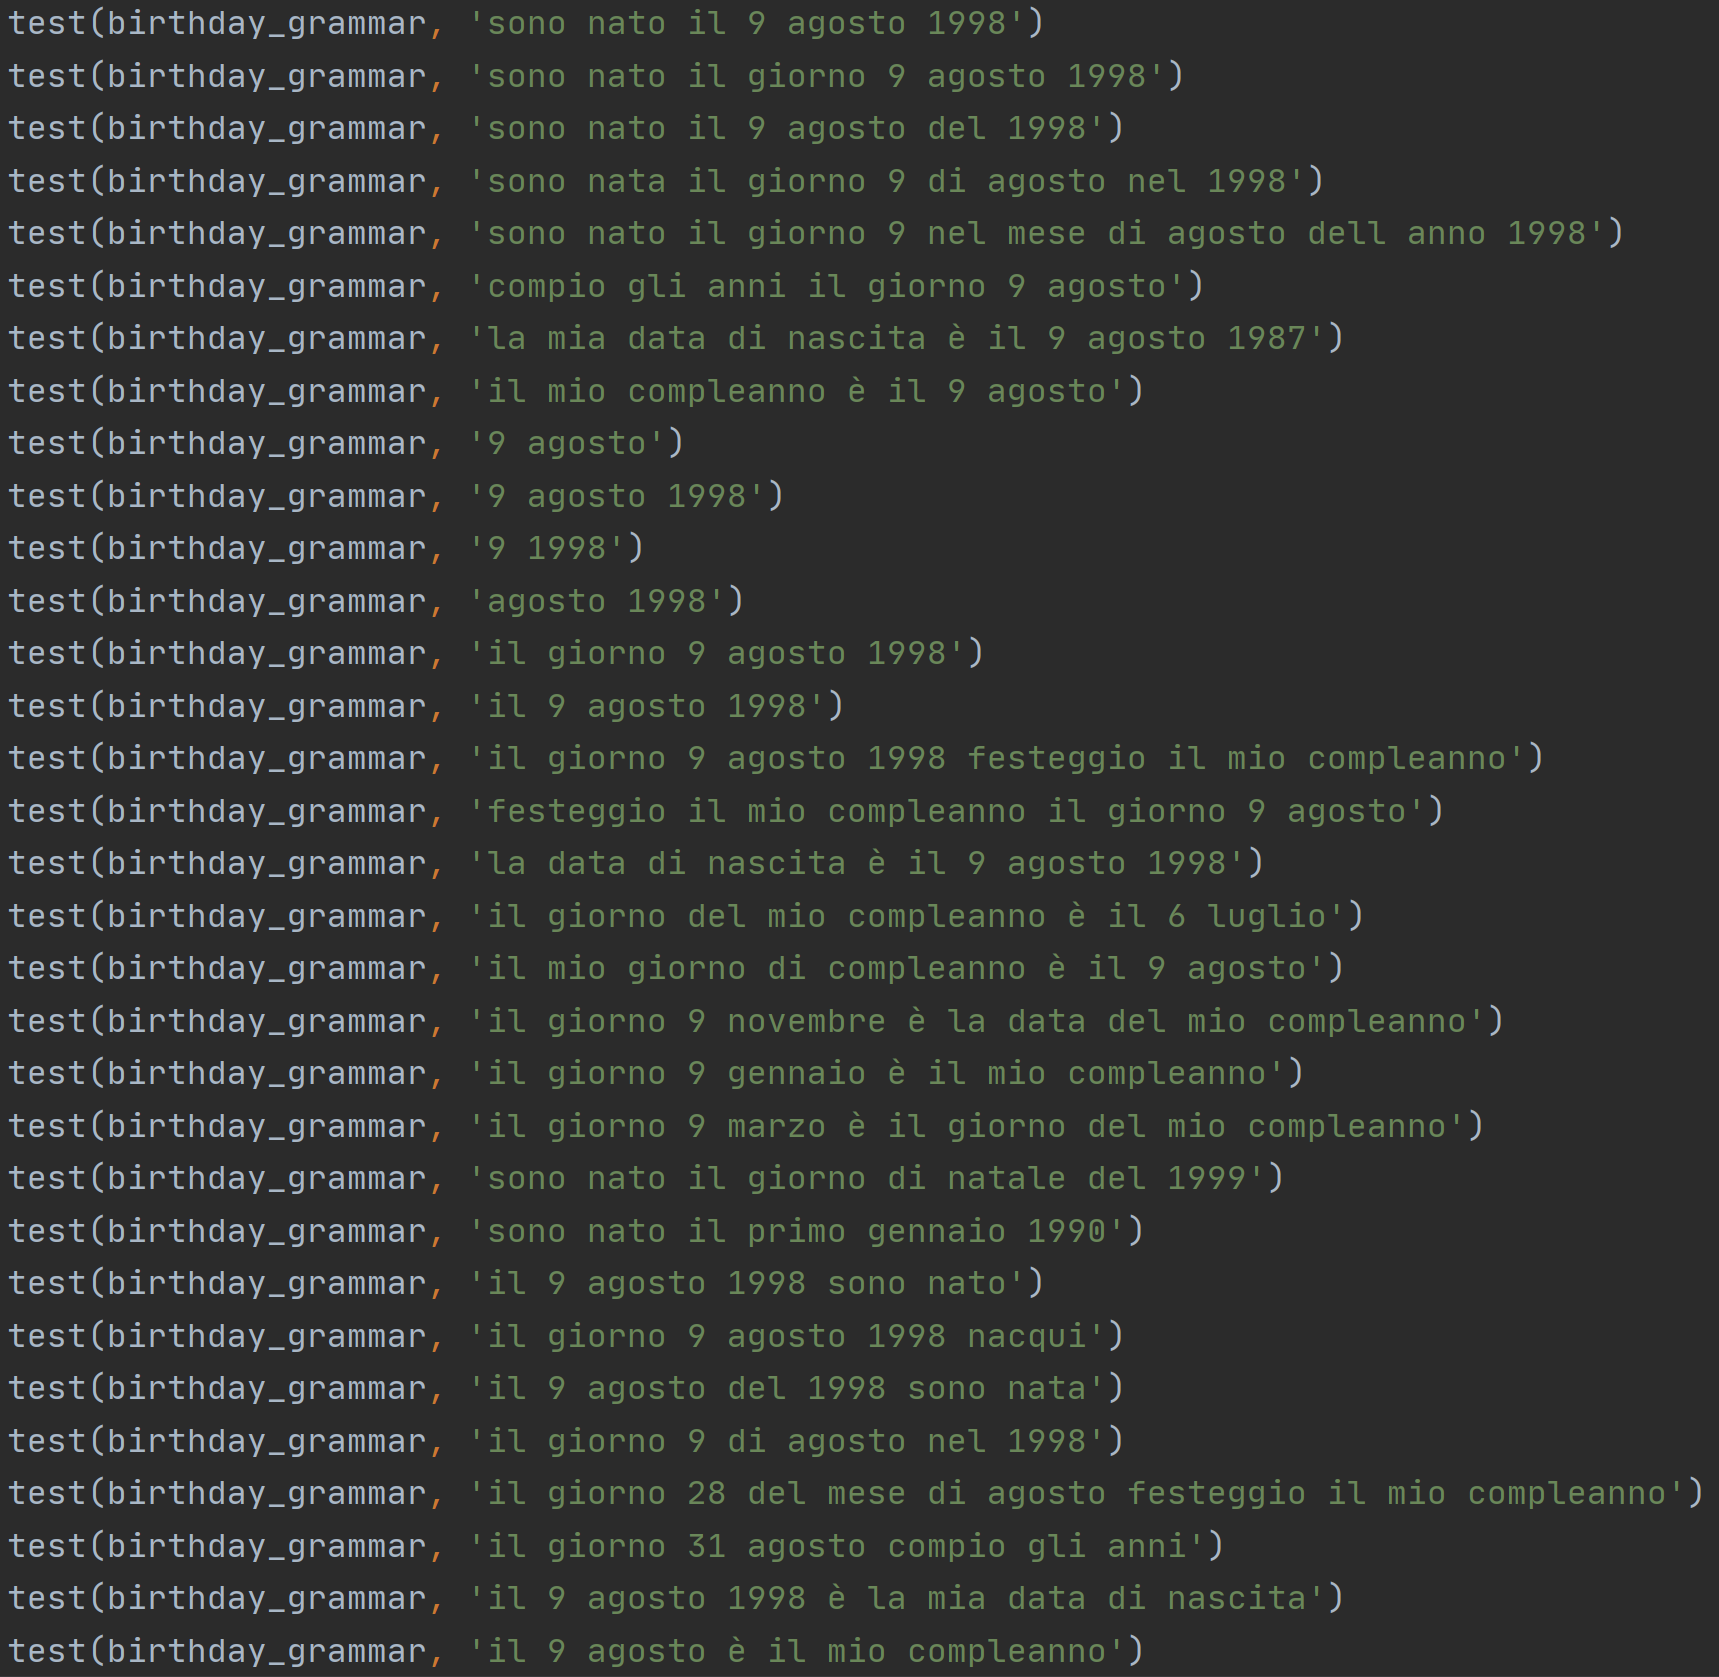
\includegraphics[height=\linewidth, width=\linewidth]{test_esempio.PNG}
		\caption{Esempio di alcune frasi di utilizzare per i test}
	\end{center}
\end{figure}
Inoltre, per verificare l'efficacia dell'interfaccia vocale, ho dato la possibilità ad utenti esterni di provare l'applicazione e ciò mi ha permesso di comprendere e sistemare numerosi difetti difficilmente riscontrabili diversamente.
\section{Risultati}
I risultati ottenuti sono stati molto positivi in quanto l'applicazione funziona correttamente ed ha soddisfatto ampiamente le aspettative dell'azienda. \\
Dato che il nucleo principale si basa sull'interfaccia vocale, è possibile visualizzare esclusivamente il riconoscimento dei comandi e le risposte all'interno della console. A questo proposito sono quindi delle figure che illustrano un esempio di conversazione. \\
Questa è la figura che rappresenta l'attività di riconoscimento dell'input con la risposta dell'applicazione. Più in dettaglio l'utente esprime solo giorno e mese di nascita e l'applicazione gli risponde confermando l'input e chiedendo l'anno di nascita per completare l'esecuzione. \\
\begin{figure}[htbp]
	\begin{center}
		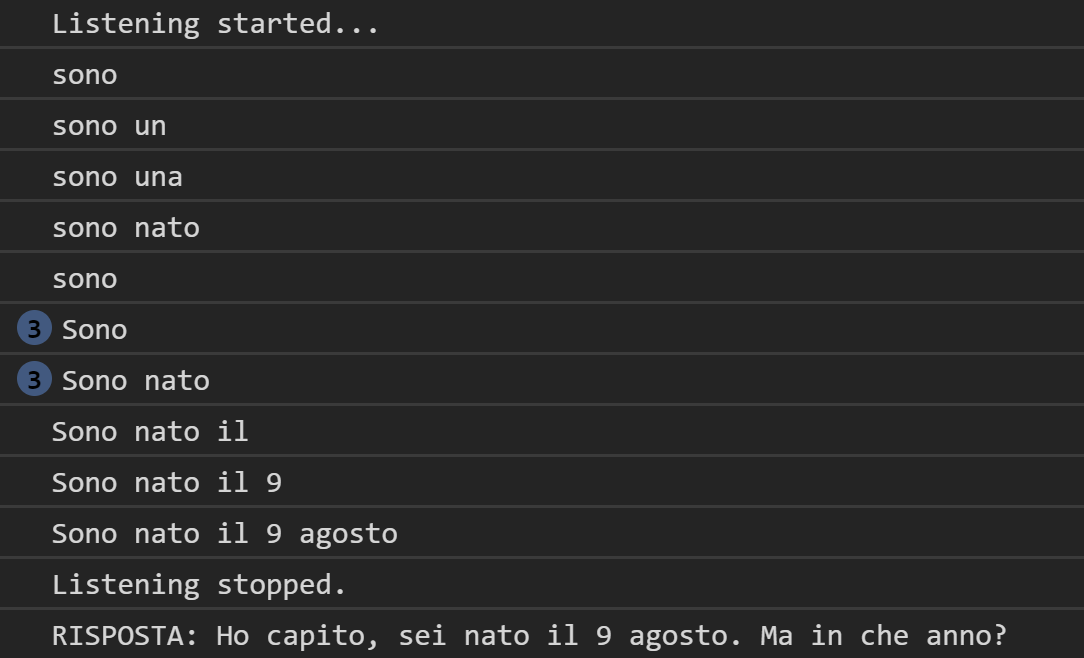
\includegraphics[height=6cm, width=9cm]{esempio-funzionamento-app-pt1.PNG}
		\caption{Esempio funzionamento applicazione: inizio conversazione}
	\end{center}
\end{figure}
\\
Questa è la figura che rappresenta il nuovo input con la risposta conclusiva dell'applicazione. Più in dettaglio l'utente esprime l'anno di nascita come richiesto e l'applicazione gli risponde confermando l'intera data di nascita e chiudendo la conversazione. \\
\begin{figure}[htbp]
	\begin{center}
		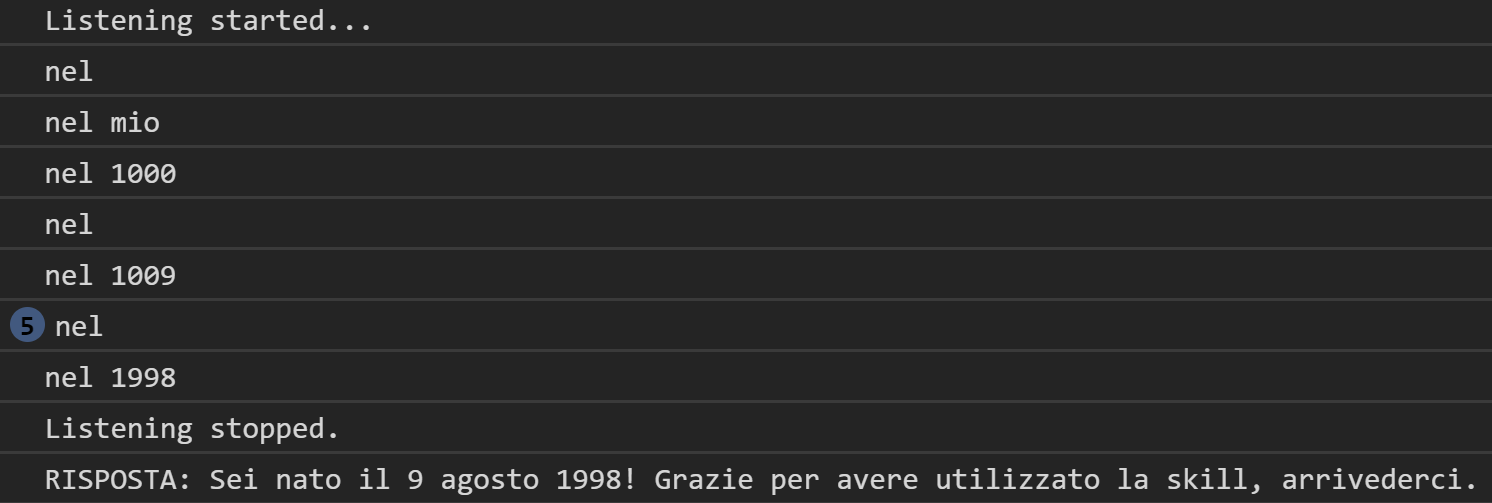
\includegraphics[height=4cm, width=9cm]{esempio-funzionamento-app-pt2.PNG}
		\caption{Esempio funzionamento applicazione: conclusione conversazione}
	\end{center}
\end{figure}
\section{Considerazioni}
Dai risultati ottenuti sono emerse delle considerazioni legate a due tematiche:
\begin{enumerate}
	\item ampliamento del contesto interpretabile dalla \emph{\gls{nlug}};
	\item utilizzo dei motori di regole per la costruzione di risposte; 
\end{enumerate}
La prima considerazione consiste nelle problematiche che comporta l'ampliamento del contesto dell'applicazione verso nuove tematiche aggiuntive e diverse dalla data di nascita. In merito a ciò la \emph{\gls{gramg}} rimane molto valida perché permette di ampliare notevolmente il contesto senza troppe difficoltà ma l'interpretazione di dati aggiuntivi rischia facilmente di diventare ambigua. In particolare mi riferisco a casi come nome e cognome in cui la \emph{\gls{nlug}} fatica a distinguerli in quanto sono entrambi stringhe talvolta interscambiabili: una stringa interpretata come un nome può essere in realtà un cognome. Una soluzione non definitiva ma accettabile entro certi limiti è la mappatura di tutte le stringhe di nomi e cognomi. Questo può essere fattibile se i domini sono piccoli, limitati e ben conosciuti ma ciò non è sempre possibile. \\
La seconda considerazione consiste nell'utilizzo di un motore di regole per la costruzione delle componenti della risposta. In generale esso permette di creare oggetti i cui parametri sono determinati da regole preconfigurate. \\
\begin{figure}[htbp]
	\begin{center}
		
\includegraphics[height=2.1cm, width=9cm]{rule-reactor.PNG}
		\caption{Logo del motore di regole}
	\end{center}
\end{figure}
\\
La sua applicazione potrebbe essere la seguente: costruire delle regole sulla base dei risultati ottenuti dall'elaborazione della \emph{\gls{nlug}} e dalla componentistica pseudo-casuale che, se saranno soddisfatte, permetteranno di costruire la risposta da ritornare all'utente sotto forma di oggetto. In questo modo rendono possibile la scrittura di codice facilmente comprensibile e manutenibile nel tempo rispetto all'utilizzo in cascata del costrutto if-else come previsto tutorial degli assistenti virtuali analizzati. Tuttavia questo motore di regole è ancora in via di sviluppo e si hanno a disposizione pochi esempi concreti.